\Section{natlog-denotations}{Denotations}
An underlying central concept behind monotonicity calculus (the natural logic used
  throughout this thesis) is the notion that lexical items can be interpreted
  in terms of their effect on the set of objects in the world.
To be precise, let's introduce a domain \sD, representing the set of all items and concepts
  in the world.
We'll show this \sD\ as an empty box:

\vspace{1em}
\begin{center}
\begin{tikzpicture}
  \frameVenn
\end{tikzpicture}
\end{center}
\vspace{1em}


Now, we can start labeling items in this set.
For example, this dissertation is an item in the world; your hand is likewise
  an item in the world.
We can write these statements as: \ww{this thesis}$ \in \sD$ and \ww{your hand}$ \in \sD$;
  visually, we might show the following:

\vspace{1em}
\begin{center}
\begin{tabular}{c@{\hskip 3cm}c}
  \begin{tikzpicture}
    \frameVenn
     \draw (0,0) node[anchor=south] {\textcolor{darkred}{\textbf{.}}};
     \draw (0.1,-0.4) node[anchor=south] {\ww{this thesis}};
  \end{tikzpicture} &
  
  \begin{tikzpicture}
    \frameVenn
     \draw (-.5,0.5) node[anchor=south] {\textcolor{darkred}{\textbf{.}}};
     \draw (0.1,0.0) node[anchor=south] {\ww{your hand}};
  \end{tikzpicture}
\end{tabular}
\end{center}
\vspace{1em}

The central dissertation behind denotational semantics is the notion that words have \textit{denotations},
  which are sets of elements in a particular domain.
For example, this dissertation and your hand have denotations which are the singleton sets of elements
  in the domain of \textit{things in the world}.
Analogously, cats will be the set of cats in the world, \ww{run} will be the set of actions which
  we'd label as running, and so forth.
The remainder of this section will go over how we map different lexical items to denotations in
  different domains.
This will form the basis of the model theory behind monotonicity calculus, introduced in
  \refsec{natlog-mono}.
%Already we are grounding bits of language (\ww{this thesis}; \ww{your hand})
%  in terms of the denotation of that language in the set $\sD$.
%This section will review a general theory for grounding arbitrary language in this
%  sort of denotational semantics.
%\todo{gabor} accumulate prior work to cite here.\needcite

% %%%%%
% Nouns and Adjectives
% %%%%%
\Subsection{natlog-denotations-nouns}{Nouns and Adjectives are Sets}
We represent nouns and adjectives as sets -- more precisely, as subsets of our domain $\sD$.
For example, the word \ww{cat} refers to the set of all cats in the world.
\ww{Cute} refers to the set of all cute things in the world.
Note that this definition subsumes the cases in the previous section: \ww{this thesis} becomes
  simply the singleton set containing this thesis.
We represent these denotations as $\llbracket cat \rrbracket \subseteq \sD$ (the set of all cats),
  $\llbracket cute \rrbracket \subseteq \sD$ (the set of all cute things), etc.
Visually, we can show these as a subset of our domain $\sD$:
  
\vspace{1em}
\begin{center}
\begin{tabular}{c@{\hskip 3cm}c@{\hskip 3cm}c}

  \begin{tikzpicture}
    \def\vennA{(-0.2,0.2) circle (0.5)}
    
    \draw \vennA node [above] {};
    \begin{scope}
      \fill[fill=dark] \vennA;
    \end{scope}
    
    \frameVenn
  \end{tikzpicture} &
  
  \begin{tikzpicture}
    \def\vennB{(0.2,-0.2) circle (0.5)}
    
    \draw \vennB node [below] {};
    \begin{scope}
      \fill[fill=dark] \vennB;
    \end{scope}
    
    \frameVenn
  \end{tikzpicture} &
  
  \begin{tikzpicture}
    \def\vennA{(-0.0,0.0) circle (0.2)}

    \draw \vennA node [above] {};
    \begin{scope}
      \fill[fill=dark] \vennA;
    \end{scope}
    
    \frameVenn
  \end{tikzpicture} \\

  $\llbracket cute \rrbracket$ &
  $\llbracket cat \rrbracket$ &
  $\llbracket this~thesis \rrbracket$

\end{tabular}
\end{center}
\vspace{1em}


%
% Don't need real interpretations
%
This is the same sort of representation used in other areas of NLP, most prominently
  the semantic parsing literature (see, e.g., \newcite{key:2015liang-potts}).
This similarity becomes more clear if we consider nouns and adjectives as
  \textit{predicates} rather than sets.
That is, the word \ww{cat} is a predicate which is true if its argument is a cat, and false
  otherwise.
These two interpretations are, of course, equivalent.
A predicate can be represented as the set of entities in the world which satisfy it,
  and a set of entities in the world can be represented as the predicate that selects them.

The key difference between denotations in monotonicity calculus and semantic parsing
  is that in the later, the world \sD\ and the denotations of words have concrete
  (domain-specific) instantiations.
For example, \sD\ may be a database of places, people, etc. that can be queried against.
In that case, the word \ww{river} would correspond to a finite set of database rows
  for the rivers in the world.
In monotonicity calculus, as we'll see more clearly in \refsec{natlog-mono}, we
  will never appeal to the explicit denotations of these lexical items.
It is sufficient to know that there exist a set of rivers in the world; we never need
  to explicitly enumerate them.


%
% Composing
%
A natural next question is how we compose lexical items into compound nouns 
  and noun phrases.
Like nouns and adjective, noun phrases are denoted as sets of object:
  \ww{cute cat} is simply the subset of items in the world which are cute cats.
\Naive ly, this composition amounts to a simple set intersection: \ww{cute cat}
  refers to the set of things which are both cats and cute;
  that is, 
  $\llbracket cute~cat \rrbracket = \llbracket cute \rrbracket \cap \llbracket cat \rrbracket$:
  

\vspace{1em}
\begin{center}
\begin{tabular}{c@{\hskip 3cm}c@{\hskip 3cm}c}
  \begin{tikzpicture}
    \def\vennA{(-0.2,0.2) circle (0.5)}
    
    \draw \vennA node [above] {};
    \begin{scope}
      \fill[fill=dark] \vennA;
    \end{scope}
    
    \frameVenn
  \end{tikzpicture} &

  \begin{tikzpicture}
    \def\vennA{(-0.2,0.2) circle (0.5)}
    \def\vennB{(0.2,-0.2) circle (0.5)}
    
    \draw[dotted] \vennB node [below] {};
    \draw[dotted] \vennA node [above] {};
    \begin{scope}
      \clip \vennA;
      \fill[fill=dark] \vennB;
    \end{scope}
    
    \frameVenn
  \end{tikzpicture} &
  
  \begin{tikzpicture}
    \def\vennB{(0.2,-0.2) circle (0.5)}
    
    \draw \vennB node [below] {};
    \begin{scope}
      \fill[fill=dark] \vennB;
    \end{scope}
    
    \frameVenn
  \end{tikzpicture} \\

  $\llbracket cute \rrbracket$ &
  $\llbracket cute~cat \rrbracket$ &
  $\llbracket cat \rrbracket$


\end{tabular}
\end{center}
\vspace{1em}


Less \naive ly, we could consider other types of composition (for more information, see
  e.g., \newcite{key:1975kamp-adjectives}).
For instance, not all adjectives behave intersectively in the way shown above.
A \ww{quick DMV visit} is still a DMV visit, but is likely not in the denotation of
  quick things.
Similarly, a \ww{small planet} is nonetheless not generally considered a \ww{small} thing.
We refer to these as \textit{subsective} adjectives -- the denotation of the compound is
  a subset of the denotation of the noun, but not a subset of the denotation of the adjective.
Another class of adjectives are outright non-subsective.
A pseudo-science is not a science; a fake gun is not a gun.
In idiomatic expressions, the denotation of the compound has nothing to do with the denotations
  of the components: a red herring is neither red nor a herring.

We'll revisit compositionality in \refsec{natlog-mono} and show that handling these sorts
  of phenomena is important to ensure that the logic remains sound.
However, for now we'll continue to review the basic components of the logic.


% %%%%%
% Sentences
% %%%%%
\Subsection{natlog-denotations-sentences}{Sentences are Truth Values}
Like most logics, the primary goal of natural logic is to assign truth
  values to sentences.
In natural logic the model-theoretic interpretation of
  a sentence is simply its truth value.
That is to say, sentences can have one of two denotations: they are either true, or they
  are false.

To make this more formal, and to lay the notational groundwork for the rest of this chapter,
  let us redefine our domain \sD\ to be $\sD_e$ -- the domain of entities in the world.
So, now, $\llbracket cat \rrbracket \subseteq \sD_e$.
We are now free to specify other domain for other types of lexical items.
In our case, let us define $\sD_t$ as the domain of truth values.
The natural way to define $\sD_t$ would be to say: $\sD_t = \{true, false\}$
  (equivalently, and as we'll find useful later, $\sD_t = \{1, 0\}$).
The denotation of a sentence is an element in $\sD_t$:

\begin{align*}
\llbracket\ww{cats eat mice}\rrbracket &= true \in \sD_t \\
\llbracket\ww{cats eat carrots}\rrbracket &= false \in \sD_t
\end{align*}

% note[gabor]: This is wrong :(
%In this dissertation we opt for this interpretation, but we should note that
%  in some formulations, $\sD_t$ is defined as a singleton set; e.g., the set $\{1\}$.
%The denotation of a sentence is then either the empty set ($\{\}$ -- corresponding to $false$)
%  or the singleton set ($\{1\}$ -- corresponding to $true$).
%The definitions are conceptually equivalent, but what we lose in clarity we gain in elegance:
%  like nouns, sentence denotations are in this case also sets:
%
%
%\begin{align*}
%\llbracket\ww{cats eat mice}\rrbracket &= \{1\} \subseteq \sD_t \\
%\llbracket\ww{cats eat carrots}\rrbracket &= \{\} \subseteq \sD_t
%\end{align*}


% %%%%%
% OTHER
% %%%%%
\Subsection{natlog-denotations-other}{Other Lexical Items are Functions}

Our review of possible linguistic phenomena or types of lexical items is by 
  no means exhaustive.
For instance, we have not covered verbs, or adverbs.
Without belaboring the chapter with pedantic thoroughness, the claim of natural logic
  is that we can construct a denotation for any of these items inductively
  from the two basic domain -- 
  the domain of entities $\sD_e$ and the domain of truth values $\sD_t$ --
  and functions based around these domains.

To begin, let's define a set $\bD_e$ to be the power set $\sD_e$: the set of all subsets
  of items in the world.
This is the set of all possible denotations.
We can then define a class of functions $f : \bD_e \rightarrow \sD_t$.
That is, the class of functions mapping from an entity to a truth value.
This corresponds most intuitively to the class of intransitive verbs: \ww{plays},
  \ww{runs}, \ww{eats}, \ww{barks}, etc.;
  it also corresponds to the denotations for longer phrases like \ww{plays chess}
  and \ww{barks at the neighbor}.
As a useful visualization, we can ``plot'' this function
  along its domain and range in  \reffig{natlog-denotation-barks}.
The $x$ axis lists the set of denotations in the world.
Recall that each of these is just an arbitrary set of items, 
  although we will label them as denotations of words.
The $y$ axis is simply the set of true and false.

\begin{figure}[h]
\begin{center}
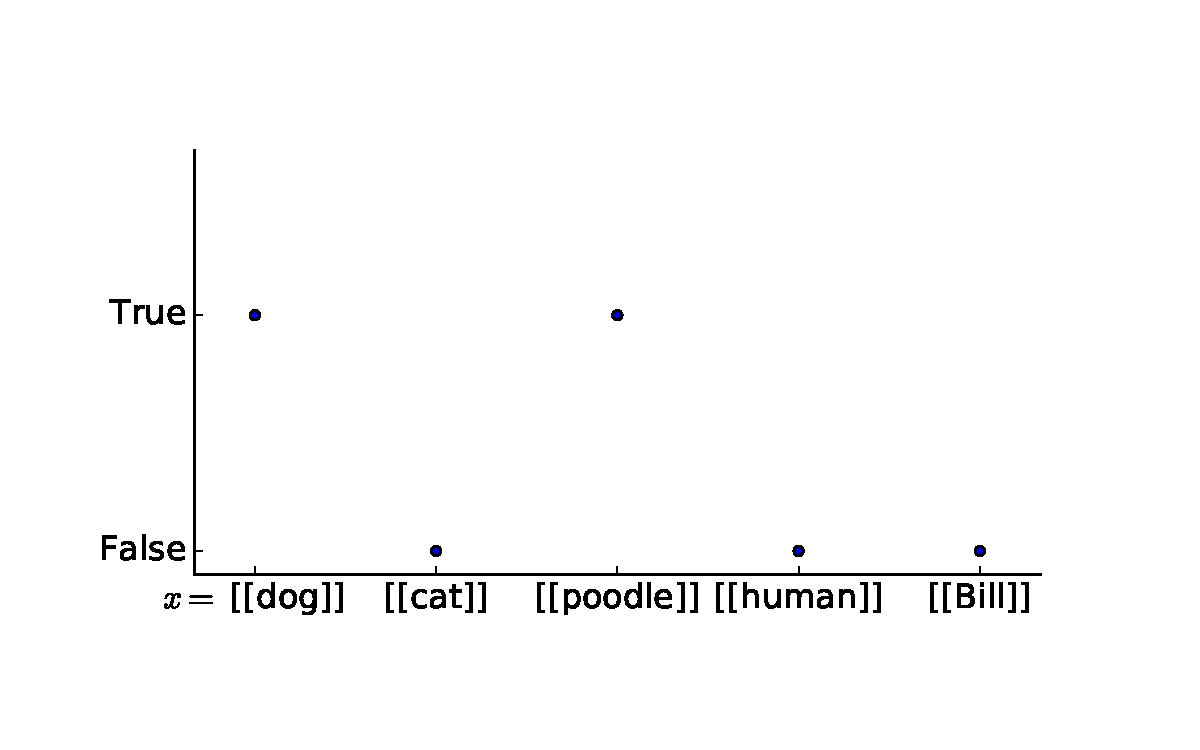
\includegraphics[height=7cm]{img/denotations_barks.pdf}
\end{center}
\caption{\label{fig:natlog-denotation-barks}
  A visualization of the denotation of \ww{barks}. The $x$ axis corresponds to denotations
  of nouns (i.e., sets of entities in the world); the $y$ axis is the domain of truth values.
}
\end{figure}

Importantly, we can keep composing functions from known domains and form new
  domains corresponding to these new functions.
For example, if the domain of intransitive functions defined above is $\sD_f$,
  we can define a class of transitive functions as $f : \sD_e \rightarrow \sD_f$.
We can alternately write this as $f : \sD_e \rightarrow (\sD_e \rightarrow \sD_t)$.
The denotation of any span of text is therefore either an entity ($\sD_e$), a truth
  value ($\sD_t$), or some class of function inductively defined above.

\paragraph{Notational Note}
It becomes tedious to write long functions as $\sD_e \rightarrow (\sD_e \rightarrow \sD_t)$;
  not to mention defining a new set for every function type, as we did for $\sD_f$.
Therefore, from now on, we'll denote the set of entities as $e = \sD_e$, the set of truth values as 
  $t = \sD_t$, and functions in the usual way of $a \rightarrow b$.
In this notational scheme, intransitive verbs are written as $e \rightarrow t$; transitive
  verbs are $e \rightarrow (e \rightarrow t)$, and so forth.


% %%%%%
% Quantifiers
% %%%%%
\Subsection{natlog-denotations-quantifiers}{Quantifiers (Operators) are Functions}

An important class of lexical items are quantifiers (and more generally natural language
  operators).
From a denotational semantics point of view, these behave just like any other function:
  \ww{all} has the same denotation as a transitive verb: $e \rightarrow (e \rightarrow t)$;
  \ww{not} has the same denotation as an intransitive verb: $e \rightarrow t$.
However, natural language operators has an important additional property: they are often
  \textit{monotonic} functions.
This property is the happy accident of language that underpins much of the usefulness
  of monotonicity calculus as a natural logic, and is the main topic of the next section.






